\section{Modification d'un corps virtuel}
Dans cette partie nous allons voir différentes méthodes pour modifier l'apparence d'un corps virtuel.

\subsection{Shape Interpolation}

La \emph{shape interpolation} permet de passer d'un modèle de corps humain à un autre en transformant les deux modèles en des ensembles de points et en calculant entre chaque point correspondant des deux modèles des points intermédiaires \cite{zh09}. Pour pouvoir réaliser cette transformation, il faut d'abord ré-échantillonner les deux modèles pour les transformer en "nuages" de points. Pour cela, un découpage du modèle est effectué en suivant l'axe du squelette du modèle. Par exemple, pour l'avant-bras une série de coupe parallèle va être réalisée en suivant la partie du squelette connectant le coude et le poignet. Le nombre de coupe réalisé sur un membre doit être identique sur les deux modèles. Une fois ceci réalisé, chaque partie du modèle est représentée par un ensemble de tranche. Ensuite le ré-échantillonnage se fait en trois étapes :
\begin{itemize}
\item \'{E}tape 1 : Pour chaque tranche, on calcule un cercle englobant cette partie du corps.
\item \'{E}tape 2 : On divise le cercle en \emph{n} sections, et on crée \emph{n} rayons qui partent du cercle et vont jusqu'au centre de la tranche.
\item \'{E}tape 3 : On crée un point à l'endroit où chaque rayon traverse la surface du modèle.
\end{itemize}
Une fois que les deux modèles ont été transformés en un ensemble de points, il faut alors calculer un ensemble de points intermédiaires. Pour cela on calcule chaque point intermédiaire de cette façon :
\begin{center}
$P = \alpha*P_i + (1-\alpha)*P_j$, avec $0<\alpha<1$
\end{center}
Avec $P$ qui est le point intermédiaire, $P_i$ et $P_j$ sont les points équivalents appartenant respectivement au modèle de départ et au modèle d'arrivée. \`{A} partir de ces points, la surface du modèle intermédiaire peut être créée en effectuant une triangulation. Sur la figure \ref{fig4} on peut voir des modèles créés avec cette technique.
\begin{figure}[!h]
   	\centerline{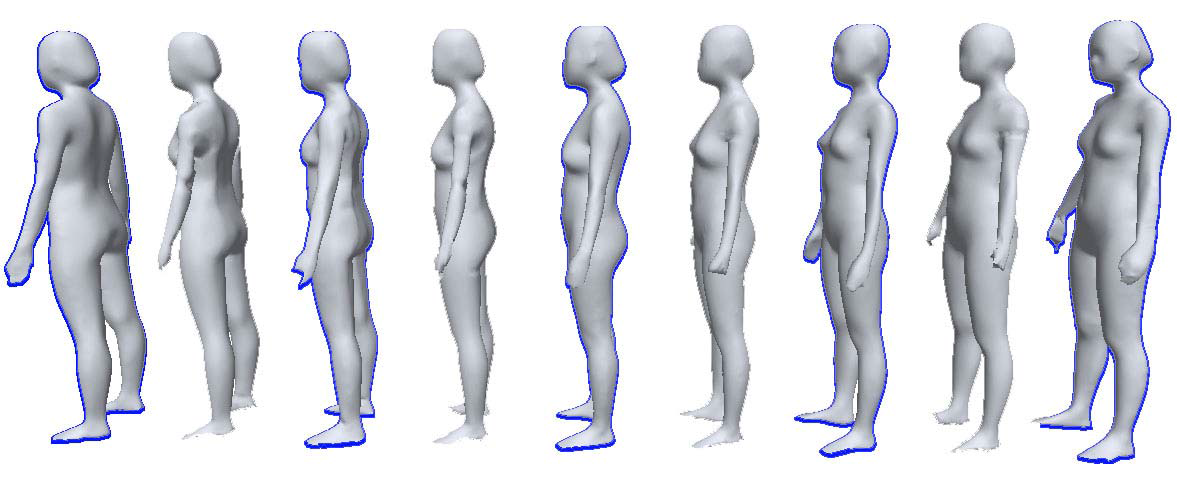
\includegraphics[scale=0.4]{./shapeInterpolation2}}
   	\caption{\label{fig4} Modèles de bases (entourés en bleu) et modèles créés par interpolation \cite{zh09}}
\end{figure}
\subsection{\emph{Morphing 3D}}
Pour réaliser un \emph{morphing} d'un humain virtuel à un autre en 3D, il faut réaliser plusieurs étapes \cite{le01} :
\begin{itemize}
\item \emph{Morphing} du squelette.
\item \emph{Morphing} de la forme.
\item \emph{Morphing} des coordonnées de la texture.
\item \emph{Morphing} de l'image de la texture.
\end{itemize}
Pour réaliser le \emph{morphing} du squelette et de la forme, il faut que les deux modèles utilisent la même structure pour définir le squelette et la forme. Ensuite les coordonnées du squelette et de la forme peuvent être calculées en utilisant une interpolation linéaire en 3D.
Pour réaliser le \emph{morphing} de la texture, il faut d'abord interpoler les coordonnées de la texture en utilisant une interpolation linéaire en 2D. Le morphing de l'image est réalisé en utilisant des techniques de triangulation. Sur la figure \ref{fig8} on peut voir des modèles créés avec cette technique.
\begin{figure}[!h]
   	\centerline{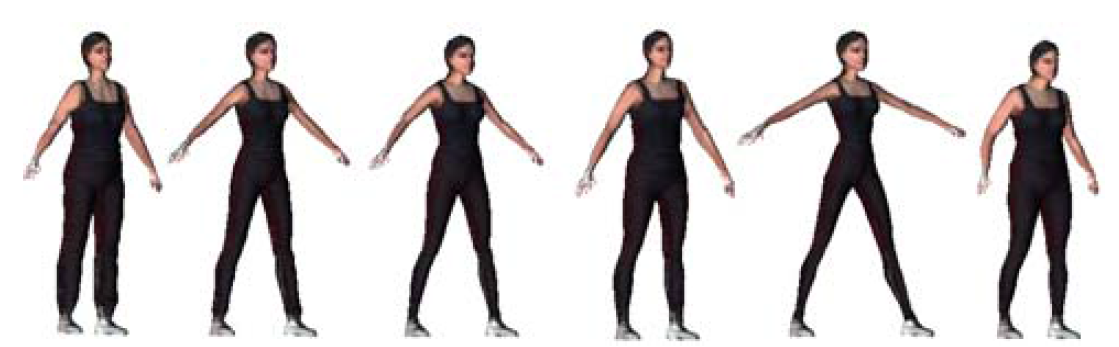
\includegraphics[scale=0.4]{./morphing}}
   	\caption{\label{fig8} Modèles avec différentes formes et la même texture \cite{le01}}
\end{figure}
\subsection{Bilan}
La \emph{shape interpolation} permet de passer d'un modèle de corps humain à un autre même si ils ne sont pas définis suivant la même structure. En effet, les points utilisés pour réaliser l'interpolation sont créés avec cette technique. Par contre, il n'y a pas de modification de la texture contrairement au \emph{morphing 3D} et le nombre de calcul est plus important que pour l'autre technique à cause du calcul des points . Comme les modèles utilisés seront connus, la structure pour définir le squelette et la forme sera identique pour les deux modèles et donc la \emph{morphing 3D} est plus approprié dans notre contexte.